Zunächsten sollen die \MatSim internen Methoden dargestellt werden.
Die Basis bildet dabei die Aerospace Toolbox von \MatSim

In Abbildung \ref{fig:Sim6DoFBlock} ist vorgefertigter Block \cite{Sim6DoFDoku}. Dieser erstellt anhand der Eulerwinkel sowie den Koordinaten $\wt{X}{e} = \begin{bmatrix}x_e &y_e &z_e \end{bmatrix}^{\textnormal{T}}$ im erdfesten Koordinatensystem eine Animation der Flugzeugbewegung.
Wie in \ref{fig:Sim6DoFBlockMenuBsp} erkennbar kann über die Blockparameter die Anzahl an Flugobjekten und deren Geometrie definiert werden. Zudem kann man den Blickwinkel und die relative Position der Kamera vorgeben. 
%\begin{figure}[h]
%	\centering
%	\begin{subfigure}[b]{0.15\textwidth}
%		\centering
%		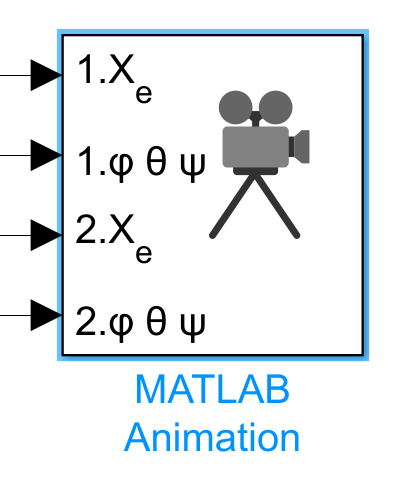
\includegraphics[width=\textwidth]{./Bilder/Visual_SimBlock.png}
%		\caption{Vorgefertigter 6DoF-Animations-Block}
%		\label{fig:Sim6DoFBlock}
%	\end{subfigure}
%	\hspace{0.1\textwidth}
%	\begin{subfigure}[b]{0.35\textwidth}
%		\centering
%		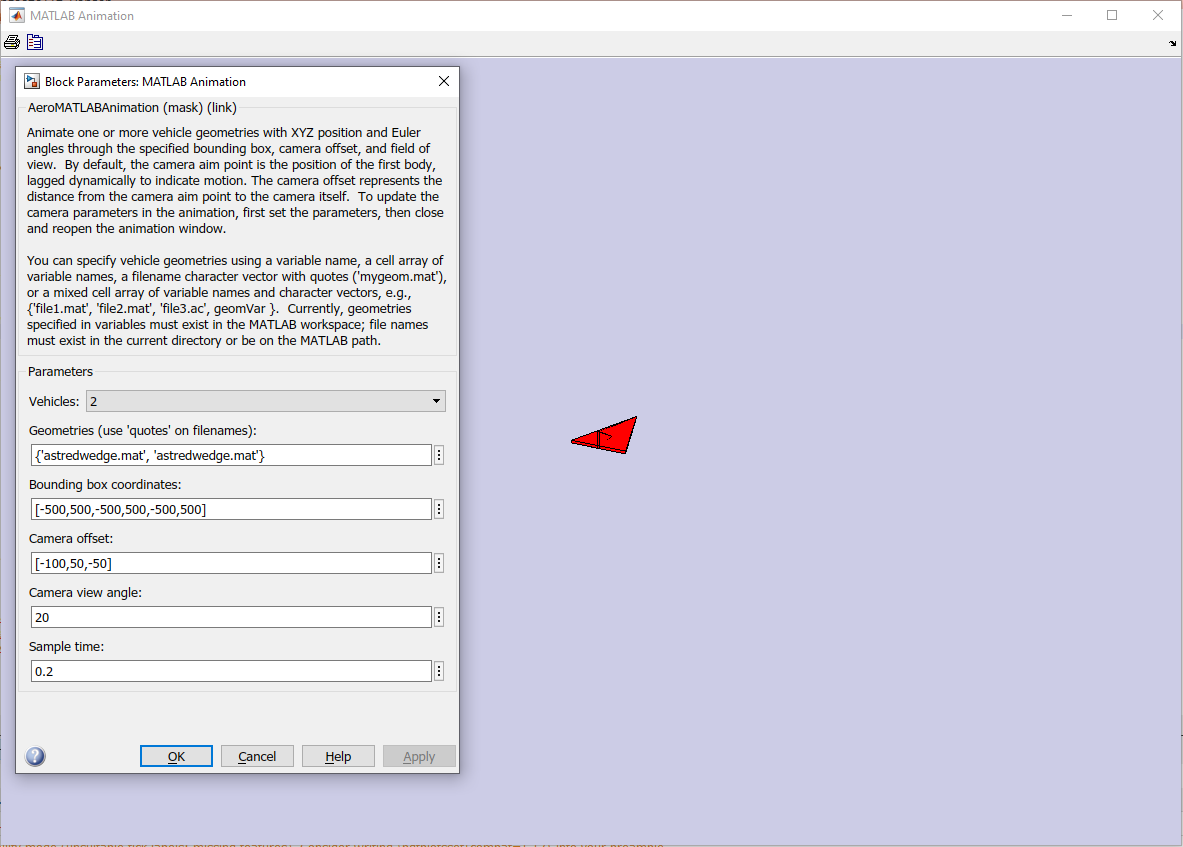
\includegraphics[width=\textwidth]{./Bilder/Visual_Sim6DoFBlockMenuBsp.png}
%		\caption{Blockparameter und Beispielanimation}
%		\label{fig:Sim6DoFBlockMenuBsp}
%	\end{subfigure}
%	\caption{Sim6DoFBlock}
%	\label{fig:Sim6DoF}
%\end{figure}
\begin{figure}[H]
	\centering
	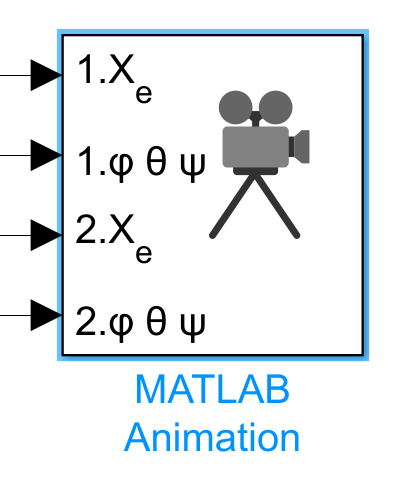
\includegraphics[width=0.35\textwidth]{./Bilder/Visual_SimBlock.png}
	\caption{Vorgefertigter 6DoF-Animations-Block in Simulink}
	\label{fig:Sim6DoFBlock}
\end{figure}

\begin{figure}[h]
	\centering
	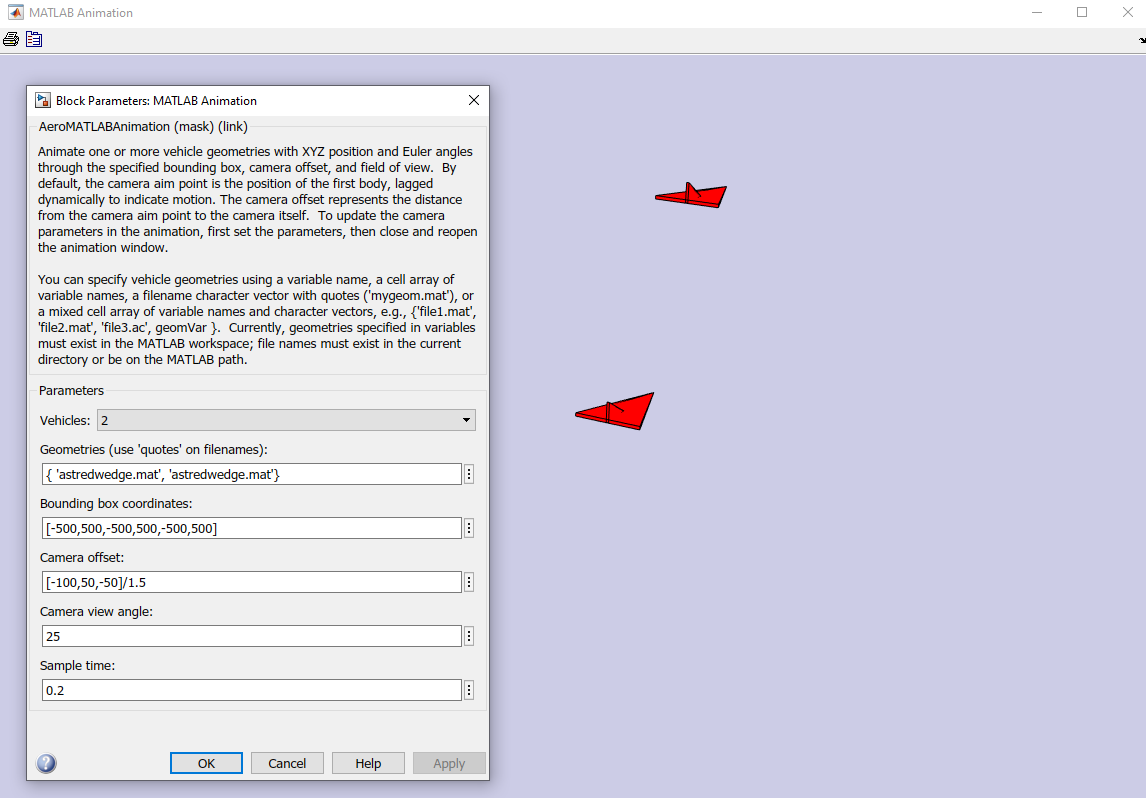
\includegraphics[width=\textwidth]{./Bilder/Visual_Sim6DoFBlockMenuBsp2.png}
	\caption{Blockparameter und Beispielanimation}
	\label{fig:Sim6DoFBlockMenuBsp}
\end{figure}
Dabei wurde für die in \ref{fig:Sim6DoFBlockMenuBsp} dargestellte Animation die voreingestellte Flugobjektgeometrie genutzt. Insgesamt betrachtet eignet sich der Animations-Block um einen Überblick über Lage, Flugbewegung und relative Position mehrerer Flugobjekte zu erhalten. Jedoch kann man die Kameraeinstellung nicht manuell während der Animation anpassen. Dies ist gerade beim Blickwinkel unpraktisch.\\
%6DoF Block:\\
%https://de.mathworks.com/help/aeroblks/6dofanimation.html\\
%Bild von Block und ergebnis\\


Eine weiter Möglichkeit der Animation bietet die Implementierung in Skriptform mit Hilfe der Aero.Animation Klasse \cite{AeroAniDoku}.
Dabei sind wieder die Flugdaten im erdfesten Koordinatensystem sowie die Eulerwinkel nötig. Zusätzlich kann über verschiedene Klassenfunktionen die Geometrie des Flugobjekts sowie die Kameraeinstellungen definiert werden. Für eine detaillierte Beschreibung der Klasse und den zugehörigen Funktionen sei auf die entsprechende Dokumentation verwiesen \cite{AeroAniDoku}.

Das in \ref{alg:MatSkripAni} dargestellte Skript beschreibt beispielhaft die Anwendung der Klasse. Der Code basiert auf dem in \cite{AeroAniOverlay} dargestellten Beispiel.
%\lstinputlisting{./inc/VisualAeroAniSkript.m}
\begin{lstlisting}[style=Matlab_colored, caption = {\Matlab-Skript zum Erstellen einer Animation über die Aero.Animation-Klasse}, label={lst:AeroAnimationSkript}]
clear;
clc;
%% Get Simulation DATA
out = sim('SixDOFSim_Vis','ReturnWorkspaceOutputs','on');
plane_1 = [out.Plane_1.time, out.Plane_1.Data];
plane_2 = [out.Plane_2.time, out.Plane_2.Data];

save('plane_1.mat', 'plane_1');
save('plane_2.mat', 'plane_2');

%% INIT Animation
% Creating instance of animation class
h = Aero.Animation; 

% Setting Framrate and Timescaling
h.FramesPerSecond = 10;
h.TimeScaling = 5;

% Creating Plane Objects
idx1 = h.createBody('pa24-250_orange.ac','Ac3d');
idx2 = h.createBody('pa24-250_blue.ac','Ac3d');

% Loading Simulation DATA
h.Bodies{1}.TimeSeriesSource = plane_1;
h.Bodies{2}.TimeSeriesSource = plane_2;

% Camera-Settings
h.Camera.PositionFcn = @doFirstOrderChaseCameraDynamics;
h.Camera.Offset = [-20,10,-10];
h.Camera.ViewAngle = 40;

% Animation
h.show();
h.play();

\end{lstlisting}

Dabei wird zunächst die Simulation gestartet um die entsprechenden Flugdaten zu erhalten. Anschließend wird eine Instanz der Animation-Klasse erzeugt. Mit Hilfe des createBody Befehls können mehrere Objekte erstellt werden. Die Geometrie wird dabei über eine entsprechende Quelldatei definiert. In dem aufgeführten Code handelt es sich bei dem Flugzeugmodel um eine Piper PA24-250 Comanche, welche von \Matlab als Beispielflugzeug genutzt wird. Ähnlich wie bei dem Animationsblock in \MatSim kann hier die Kameraeinstellungen durch relative Position und Blickwinkel bestimmt werden.

Ein Frame, der sich daraus ergebende Animation, ist in Abbildung \ref{VisualMatSk2Plane} dargestellt.
\begin{figure}[h]
	\centering
	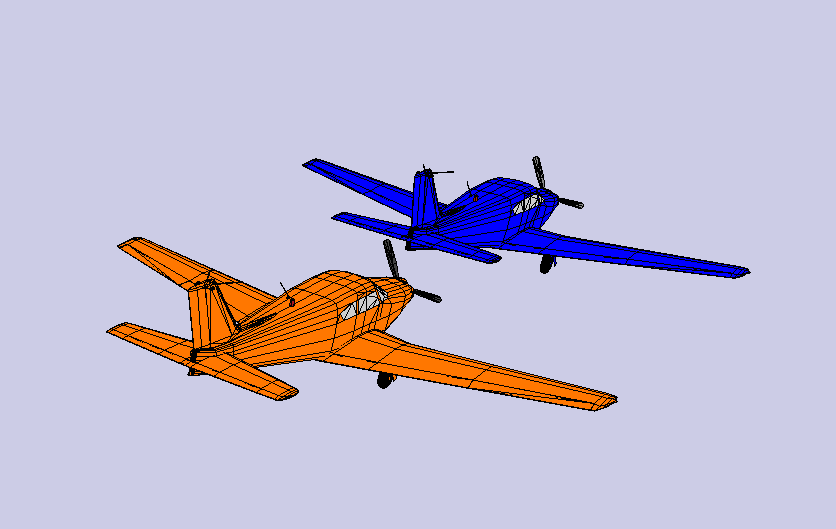
\includegraphics[width=\textwidth]{./Bilder/VisualMatSk2Plane.png}
	\caption{Beispielanimation mit Hilfe der Aero.Animaiton-Klasse}
	\label{fig:VisualMatSk2Plane}
\end{figure}
Auch hier sind die Flugbewegungen übersichtlich darstellbar aber eine handliche Anpassung des Blickwinkels ist wieder nicht gegeben.

Beide Methoden eigen sich um die relativen Bewegungen der beiden Flugzeuge zu veranschaulichen. 
Da jedoch jeweils kein Horizont oder Hintergrundobjekte implementiert sind, ist die global Flugbewegung nur schwer nachvollziehbar.


%Als Matlabskript:\\
%Ein Flugzeug:
%Skript
%Bild von zwei Flugzeugen 

%Einfache Erweiterung um weiter Flugzeuge:
%	-> Overlaying :\\
%	https://de.mathworks.com/help/aerotbx/ug/overlaying-simulated-and-actual-flight-data.html
	

%Zitate:\\
%https://de.mathworks.com/help/aerotbx/ug/aero.animation-class.html 						LABEL: AeroAniDoku\\
%https://de.mathworks.com/help/aerotbx/ug/overlaying-simulated-and-actual-flight-data.html	LABEL: AeroAniOverlay\\
%https://de.mathworks.com/help/aeroblks/6dofanimation.html									LABEL: Sim6DoFDoku\\
